\chapter{The Mechanical Way Of Living}

This chapter follows J. Krishnamurti's Brockwood Park dialogue on psychological security, mechanical order, fear, and time. The source material belongs to the Krishnamurti Foundation Trust corpus and is curated here by LazyingArt LLC through the Video2Book course project. There are no retained blackboard equations, diagrams, or mathematical screenshots for this lecture; the displayed formulae and TikZ figures are therefore transcript-grounded schematics, not visual transcriptions. Their purpose is to keep the order of the inquiry visible: security becomes belief, belief becomes image, image requires occupation, and occupation becomes a mechanical way of living.

\section{The Unfinished Question: Is Psychological Security Real?}

The dialogue opens as a continuation. The previous discussion had accepted that psychological security is a delusion, but one participant says that the reason was not made clear enough. That is the right place to begin, because psychological security does not ordinarily appear as an abstract error. It appears necessary. A frightened, sorrowful, or disturbed person may feel that some inward security must be established before anything else can be done.

Krishnamurti's first move is not to offer consolation, and not to dismiss the need. He asks the prior question:

\begin{equation}
\text{Is there psychological security at all?}
\end{equation}

The answer cannot be rushed, because the assumption of psychological security is already built into the questioner. We think we have it, or can obtain it, or would collapse without it. So the inquiry pauses over the meaning of the term. Psychological security is described as permanency, stability, continuity, and a deep-rooted sense of inner existence. It is something to count on, cling to, hold to, or treat as imperishable.

A first schematic of the opening movement is:

\begin{equation}
\text{conditioning}
\longrightarrow
\text{search for security}
\longrightarrow
\text{clinging}
\longrightarrow
\text{threat}
\longrightarrow
\text{insecurity}.
\end{equation}

The point is not that conditioning is one external cause among others. The point is that we are trained to give importance to psychological security, and then the object of dependence becomes a source of fear. What one clings to can be disturbed.

\begin{table}
\centering
\begin{tabular}{|p{0.30\linewidth}|p{0.58\linewidth}|}
\hline
\textbf{Term} & \textbf{Working meaning in the dialogue} \\
\hline
Physical security & Bodily and material safety; necessary, but not the central object of the critique. \\
\hline
Psychological security & The inward demand for permanency, continuity, and something imperishable to depend on. \\
\hline
Belief & A projected support that gives comfort, continuity, or a sense that life will finally come right. \\
\hline
Image & A picture, symbol, or conclusion through which one sees oneself, another person, work, or relationship. \\
\hline
Conclusion & The psychological surplus added by thought to actual facts. \\
\hline
Occupation & More than doing tasks; psychological absorption that keeps the brain in an apparently ordered state. \\
\hline
Mechanical order & Repetitive order that gives temporary safety but remains fragile, dull, and disturbed. \\
\hline
Actual perception & Direct seeing of what is so, distinguished from abstract assent. \\
\hline
\end{tabular}
\caption{The main distinctions needed for the inquiry into security and mechanical living.}
\end{table}

\section{From Permanency To Becoming}

The conversation then collects examples. A person believes in heaven and feels that present suffering is temporary. Another believes that communism will solve everything in time. A scientist may feel secure in the discovery of permanent laws. A doctor may feel secure in knowledge, routine, patients, position, and professional recognition. A mother may feel secure in the child. Gold appears as an old symbol of the imperishable: something that does not corrode and can be counted on.

The examples are deliberately ordinary. We are not comparing doctrines; we are watching the same structure appear in different materials. The general form is:

\begin{align}
\text{belief}+\text{continuity} &\longrightarrow \text{comfort}, \\
\text{knowledge}+\text{status} &\longrightarrow \text{felt permanence}, \\
\text{property}+\text{attachment} &\longrightarrow \text{something to hold on to}.
\end{align}

But this kind of security contains conflict from the beginning. If it depends on work, illness or failure may disturb it. If it depends on another person, the relationship may alter. If it depends on belief, the belief must be maintained. Therefore the thing that promises stability becomes the thing that must be protected.

The next turn is more subtle. Security is not only having something. It is also anticipating something. If the present is lonely, disappointing, painful, or uncertain, thought projects a future in which life will be better. The future image gives comfort now.

\begin{equation}
\text{present discomfort}
+
\text{anticipated future safety}
\longrightarrow
\text{felt security now}.
\end{equation}

So security is redescribed as becoming. The form is not merely, ``I have something permanent.'' It is also, ``I shall become safe,'' ``I shall be loved,'' ``I shall be successful,'' or ``life will come right.'' The patient will find someone to love him; the professional will become important; the religious believer will reach a permanent state; the ambitious person will become chief, famous, or fulfilled. The notation is compact:

\begin{equation}
\text{psychological security}
\sim
\text{becoming better in psychological time}.
\end{equation}

The sign \(\sim\) is deliberate. It marks an affinity in the dialogue, not a formal identity. Krishnamurti is exposing the movement by which the present borrows comfort from an imagined future.

\subsection{Question \& Answer}

\paragraph{Question.}
If there is no psychological security, does that mean there is no psychological tomorrow? And if there is no psychological tomorrow, has hope been taken away?

\paragraph{Answer.}
The dialogue does not replace one hope with another. It distinguishes practical tomorrow from psychological tomorrow. Practical tomorrow is necessary: appointments, work, food, travel, learning a language, repairing a house. Psychological tomorrow is different. It is the projected future in which the self becomes more secure, more loved, more successful, more complete.

\begin{align}
\text{practical tomorrow} &: \text{chronological arrangement and skill}, \\
\text{psychological tomorrow} &: \text{projected becoming of the self}.
\end{align}

The challenge falls on the second line. If security means the certainty that the self will become safe in time, the lecture asks whether such security exists in actuality.

\section{Idea, Fact, And Perception}

At this point the inquiry refuses a merely empirical answer. We can say that death comes, that everything changes, that one cannot count on health, money, relationship, feeling, or social position. The speakers acknowledge all this. But Krishnamurti calls it superficial for the present purpose. The deeper question is why the fact does not act as fact.

A person can hear, ``there is no psychological security,'' and convert it into an idea. The idea may be correct, but the old movement continues. This gives the lecture one of its central distinctions:

\begin{equation}
\text{idea} \not\Rightarrow \text{action},
\qquad
\text{perception} \Rightarrow \text{action}.
\end{equation}

We should read this as a disciplined shorthand, not as a theory of mind. Abstract agreement does not end the movement of seeking security. Direct perception is different. If one actually sees the clinging, action is not a separate method added afterward. In Krishnamurti's phrase, action comes through perception, not through ideation.

\subsection{Question \& Answer}

\paragraph{Question.}
Why does ``there is no security'' become an idea instead of an actual fact, like a table, a hand, or a flower?

\paragraph{Answer.}
Because the self that seeks security appears to itself as real. If the self is taken as an actual center, then it must protect itself. The statement that there is no security threatens that center. Thought therefore turns the fact into an idea. As an idea it can be considered, accepted, repeated, resisted, or refined without ending the underlying movement.

The distinction is:

\begin{align}
\text{abstract assent} &: \text{``I understand there is no security''}, \\
\text{actual perception} &: \text{seeing the clinging as it operates}.
\end{align}

This is why the dialogue keeps correcting premature action. The question is not yet, ``How do I destroy the need for security?'' That already assumes a method and a future. The first question is whether the movement is actually seen.

\section{Image, Conclusion, And The Doctor Example}

The middle of the dialogue turns from security to image. If security lies in belief, profession, relationship, symbol, or conclusion, then one sees the world through that structure. A wife, patient, colleague, house, ideology, or religious belief is no longer simply met; each is fitted into the function it serves for the self.

The point is stated sharply: the picture, the image, the conclusion is the security. Then the speakers ask why this image becomes so fantastically real. It can seem more real than the hills, the marble, or the physical objects in front of them. The abstract proof that there is no security does not penetrate it, because the image presents itself as the solid reality of ``me.''

The doctor example makes the distinction concrete. We may write:

\begin{equation}
\text{doctor identity}
=
\text{actual function}
+
\text{psychological conclusion}.
\end{equation}

Expanding the two terms gives:

\begin{align}
\text{actual function}
&=
\text{training}
+
\text{knowledge}
+
\text{daily operation}, \\
\text{psychological conclusion}
&=
\text{status}
+
\text{comparison}
+
\text{continuity}
+
\text{fear of loneliness}.
\end{align}

Training took place. Knowledge has been acquired. Patients are seen. Work is done. These are actual. But thought adds a conclusion: ``I am a doctor'' as identity, importance, comparison, and protection from being nothing or alone.

\begin{table}
\centering
\begin{tabular}{|p{0.42\linewidth}|p{0.42\linewidth}|}
\hline
\textbf{Actual in the example} & \textbf{Added by conclusion} \\
\hline
Training & Status and professional self-image \\
\hline
Knowledge & Comparison with others \\
\hline
Daily operation & Continuity of identity as ``me'' \\
\hline
Seeing patients & Fear that without this there is no activity \\
\hline
Functional skill & Protection from loneliness or emptiness \\
\hline
\end{tabular}
\caption{The doctor example separates actual function from the psychological surplus attached to identity.}
\end{table}

The worked sequence is:

\begin{enumerate}
\item There are actual facts: training, knowledge, and daily operation.
\item Thought gathers those facts into the conclusion, ``I am this.''
\item The conclusion becomes a source of status, continuity, and protection.
\item The person acts to maintain the conclusion.
\item The conclusion therefore requires occupation; without occupation, loneliness and fear return.
\end{enumerate}

This is the hinge into the title theme. The self-image cannot merely sit there. It has to be kept in motion. It needs a process.

\section{Occupation And Mechanical Order}

Occupation now becomes the practical center of the lecture. The word does not mean only being busy. It means that the brain is absorbed in a content that gives it a sense of order. One may be seeing patients, writing books, doing arithmetic, running a house, going to the laboratory, joining a community, or seeking entertainment. The activity may differ; the psychological function is the same.

The encephalograph story is used only as an anecdote in the transcript. A disturbed woman is said to show a wild pattern until she is occupied with arithmetic; then the pattern becomes smooth; when she stops, it becomes wild again. Since no visual trace is retained, we do not draw an EEG waveform. We keep only the transcript-backed structure:

\begin{equation}
\text{unoccupied brain}
\longrightarrow
\text{instability}
\longrightarrow
\text{occupation}
\longrightarrow
\text{mechanical order}.
\end{equation}

The phrase ``mechanical order'' is exact. There is order in occupation, but it depends on the continuation of the mechanism. It works for a time. Then boredom, dullness, interruption, or threat appears. The person seeks another occupation, another interest, another habit, another structure.

\begin{equation}
\text{mechanical order}
=
\text{disorder masked as order}.
\end{equation}

This equality is a conceptual compression of the dialogue. It should not be read as a proven identity in a formal system. It preserves the moment when the speakers see that the apparent order contains conflict because it depends on conditions continuing.

\begin{figure}
\centering
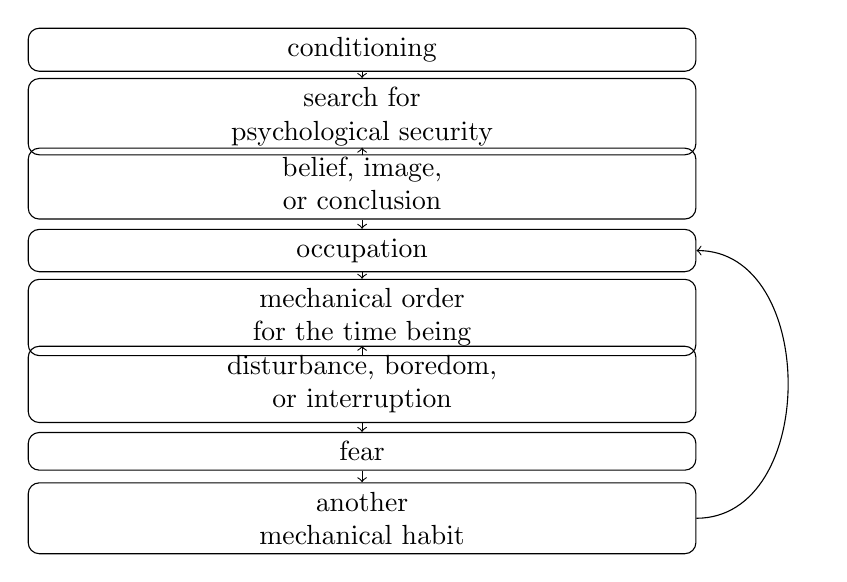
\begin{tikzpicture}[node distance=0.85cm]
\node[draw, rounded corners, align=center, text width=0.68\linewidth] (a) {conditioning};
\node[draw, rounded corners, align=center, text width=0.68\linewidth, below of=a] (b) {search for\\psychological security};
\node[draw, rounded corners, align=center, text width=0.68\linewidth, below of=b] (c) {belief, image,\\or conclusion};
\node[draw, rounded corners, align=center, text width=0.68\linewidth, below of=c] (d) {occupation};
\node[draw, rounded corners, align=center, text width=0.68\linewidth, below of=d] (e) {mechanical order\\for the time being};
\node[draw, rounded corners, align=center, text width=0.68\linewidth, below of=e] (f) {disturbance, boredom,\\or interruption};
\node[draw, rounded corners, align=center, text width=0.68\linewidth, below of=f] (g) {fear};
\node[draw, rounded corners, align=center, text width=0.68\linewidth, below of=g] (h) {another\\mechanical habit};
\draw[->] (a) -- (b);
\draw[->] (b) -- (c);
\draw[->] (c) -- (d);
\draw[->] (d) -- (e);
\draw[->] (e) -- (f);
\draw[->] (f) -- (g);
\draw[->] (g) -- (h);
\draw[->] (h.east) .. controls +(1.55,0.0) and +(1.55,0.0) .. (d.east);
\end{tikzpicture}
\caption{A transcript-grounded reconstruction of mechanical security. No screenshot accompanies it because no useful board or diagram frame was validated for this lecture.}
\end{figure}

\subsection{Question \& Answer}

\paragraph{Question.}
Why does the brain seem to go wild when it is not occupied, and why does mechanical order fail to be real order?

\paragraph{Answer.}
In occupation there is a kind of order because the brain has content, direction, and repetition. But that order is only mechanical. It depends on the continuity of the process. When the occupation stops, instability returns. If the process continues too long, boredom or dullness appears. If the process is threatened, fear appears. So the order is not free from disorder; it is a way of holding disorder in place.

A cautious update rule makes the movement clear:

\begin{equation}
M_{n+1}
=
\begin{cases}
M_n, & \text{while the mechanism gives order for the time being},\\
M_{\mathrm{new}}, & \text{when disturbance, boredom, or fear appears}.
\end{cases}
\end{equation}

Here \(M_n\) denotes the current mechanical process, and \(M_{\mathrm{new}}\) denotes the next habit or occupation. This is only a notation for the spoken sequence. It is not a formal psychology. Its value is that it shows why moving from one occupation to another can still be the same mechanical movement.

\section{Why The Brain Remains Mechanical}

The later dialogue asks a sharper question: why does the brain become mechanical, and why does it remain mechanical? The first answers are partial. Mechanical living is repetitious. It is action and reaction. It is easy. It gives a boundary. It seems safe. But Krishnamurti presses further.

The brain wants order. Without order it cannot function properly. Since mechanical order is safe for the time being, the brain accepts it and hopes it will not end in disaster. That phrase, ``for the time being,'' is important. The mechanical process does give a temporary order; otherwise the brain would not accept it. But temporary order is not total order.

\begin{align}
\text{brain needs order}
&\longrightarrow
\text{accepts mechanical process}, \\
\text{mechanical process disturbed}
&\longrightarrow
\text{fear of collapse}, \\
\text{fear of collapse}
&\longrightarrow
\text{renewed mechanism}.
\end{align}

Conditioning reinforces the pattern. Tradition, education, culture, childhood obedience, professional reputation, belief, and community all train the brain to find order mechanically. Even revolt can remain mechanical: one leaves a profession, belief, or routine and enters another structure that works in the same way.

The central late proposition can be stated as follows.

\begin{proposition}
The mechanical way of living leads to disorder, even though it is adopted in the hope of order.
\end{proposition}

\begin{proof}
This is not a formal proof in the mathematical sense; it is the ordered argument of the dialogue.
\begin{enumerate}
\item The brain needs order in order to function.
\item It accepts a mechanical process because that process gives order for the time being.
\item The process depends on repetition, continuity, and conditions remaining in place.
\item Life disturbs those conditions.
\item When the mechanism is disturbed, fear appears.
\item To escape that fear, the brain establishes another mechanical habit.
\item Therefore the original order was not total order; it was disorder maintained under the appearance of order.
\end{enumerate}
\end{proof}

This is where the dialogue becomes especially delicate. Krishnamurti says that if the whole movement is seen, there is instant action and an order that is not fragmented. A participant immediately objects that this does not yet follow logically. The objection must remain in the chapter. The lecture does not present ``indestructible order'' as a completed theorem. It says the matter can be gone into only if the mechanical security developed, attached to, and cultivated by the brain is actually perceived.

\section{When The Past Meets The Present}

The final movement brings the whole inquiry into time and relationship. We meet another person through memories, images, reputation, words, pictures, and symbols. With that past, we meet the person now. This is the phrase the dialogue settles on: the past meets the present.

\begin{equation}
\text{past}
=
\{\text{memory},\text{image},\text{reputation},\text{word},\text{picture},\text{symbol}\}.
\end{equation}

If the past continues through the present, relationship is mediated by image. The other person may have changed, but the old memory meets him. In that case one does not meet the person; one meets the past. Krishnamurti says that when this movement continues, it is one of the factors of time movement, bondage, fear, and disorder.

\begin{equation}
\text{past meets present and continues}
\longrightarrow
\text{time movement}+\text{bondage}+\text{fear}.
\end{equation}

The alternative is not a technique for suppressing memory. The dialogue is more exact than that. It asks whether the movement of the past meeting the present can be completely observed. If it is fully observed, Krishnamurti says, the movement stops. Then there is the possibility of meeting the other as though for the first time.

\begin{equation}
\text{complete awareness of the movement}
\longrightarrow
\text{the movement stops}.
\end{equation}

\begin{figure}
\centering
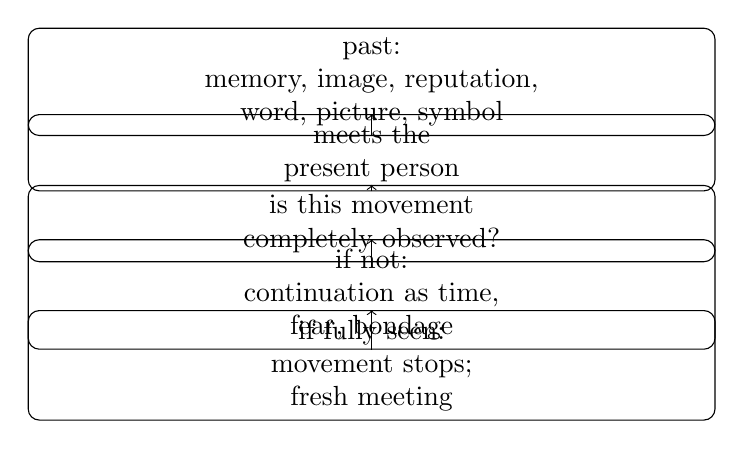
\begin{tikzpicture}[node distance=0.90cm]
\node[draw, rounded corners, align=center, text width=0.70\linewidth] (past) {past:\\memory, image, reputation,\\word, picture, symbol};
\node[draw, rounded corners, align=center, text width=0.70\linewidth, below of=past] (meet) {meets the\\present person};
\node[draw, rounded corners, align=center, text width=0.70\linewidth, below of=meet] (observe) {is this movement\\completely observed?};
\node[draw, rounded corners, align=center, text width=0.70\linewidth, below of=observe] (no) {if not:\\continuation as time,\\fear, bondage};
\node[draw, rounded corners, align=center, text width=0.70\linewidth, below of=no] (yes) {if fully seen:\\movement stops;\\fresh meeting};
\draw[->] (past) -- (meet);
\draw[->] (meet) -- (observe);
\draw[->] (observe) -- (no);
\draw[->] (no) -- (yes);
\end{tikzpicture}
\caption{The late relationship structure: the past meets the present; if it continues, it becomes time and fear; if fully observed, the movement may stop.}
\end{figure}

The ending is intentionally unfinished. The speakers say they have not really tackled the root: the disturbance, turmoil, travail, anxiety, and wild disorder of the brain. The final question is not decorative. It is the question left for the next inquiry: why do human beings live this way? The final answer named in the dialogue is brief and double: time.

\section{Summary}

The lecture begins with an unfinished question about psychological security and ends with the root problem of time. Its progression is precise. Security is first examined as belief, knowledge, status, property, relationship, and tradition. It is then seen as becoming: the hope that the future will make the self safe. The discussion then turns from idea to fact, from fact to perception, from perception to image, from image to occupation, from occupation to mechanical order, and from mechanical order to the past meeting the present.

The compact chain is:

\begin{equation}
\text{security}
\longrightarrow
\text{image}
\longrightarrow
\text{occupation}
\longrightarrow
\text{mechanical order}
\longrightarrow
\text{disorder}
\longrightarrow
\text{time}.
\end{equation}

The diagrams and equations in this chapter are deliberately modest. They do not formalize Krishnamurti into a theory. They preserve the steps of the lecture so that the reader can see the movement unfold: the search for security creates the structure that must be defended, and the defense of that structure becomes the mechanical way of living.